\section{Слежение и компенсация}
\subsection{Задание сигнала}
Зададим сигнал $f$, состоящий из пяти гармоник следующим образом:
\begin{equation}
    f(t) = \sum_{i=1}^{5} A_i \cos(\omega_i t + \phi_i)
\end{equation}
Запишем систему, описывающую генератор внешнего возмущения: 
\begin{equation}
    \begin{cases}
        \dot{\omega}_f = \Gamma_f \omega_f \\
        f = Y_f \omega_f
    \end{cases}
\end{equation}
где $\Gamma_f$ -- матрица гармоник, $Y_f$ -- матрица весов. 

Таким образом, для задания внешнего возмущения $f(t)$ необходимо задать матрицы 
$\Gamma_f$, $Y_f$ и начальное значение $w_f(0)$. 

Пусть матрица $\Gamma_f$ имеет вид:
\begin{equation}
    \Gamma_f = \begin{bmatrix}
        0 & -1 & 0 & 0 & 0 & 0 & 0 & 0 & 0 & 0 \\
        1 & 0 & 0 & 0 & 0 & 0 & 0 & 0 & 0 & 0 \\
        0 & 0 & 0 & -2 & 0 & 0 & 0 & 0 & 0 & 0 \\
        0 & 0 & 2 & 0 & 0 & 0 & 0 & 0 & 0 & 0 \\
        0 & 0 & 0 & 0 & 0 & -3 & 0 & 0 & 0 & 0 \\
        0 & 0 & 0 & 0 & 3 & 0 & 0 & 0 & 0 & 0 \\
        0 & 0 & 0 & 0 & 0 & 0 & 0 & -4 & 0 & 0 \\
        0 & 0 & 0 & 0 & 0 & 0 & 4 & 0 & 0 & 0 \\
        0 & 0 & 0 & 0 & 0 & 0 & 0 & 0 & 0 & -5 \\
        0 & 0 & 0 & 0 & 0 & 0 & 0 & 0 & 5 & 0 \\
    \end{bmatrix}
\end{equation}

Матрица весов $Y_f$ может быть задана как:
\begin{equation}
    Y_f = \begin{bmatrix}
        0.3 & -0.5 & 0.2 & -1.0 & 0.9 & 0.4 & 0.6 & 0.8 & -0.7 & 0.1 \\
    \end{bmatrix}
\end{equation}
и начальное значение $w_f(0)$:
\begin{equation}
    w_f(0) = \begin{bmatrix}
        1.0 & 0 & 0 & 0 & 0.3 & 0 & 0 & 0 & 0.5 & 0 \\
    \end{bmatrix}^T
\end{equation}

Промоделируем полученную систему. Результат моделирования представлен на рисунке \ref{fig:signal_generation}.
\begin{figure}[ht!]
    \centering
    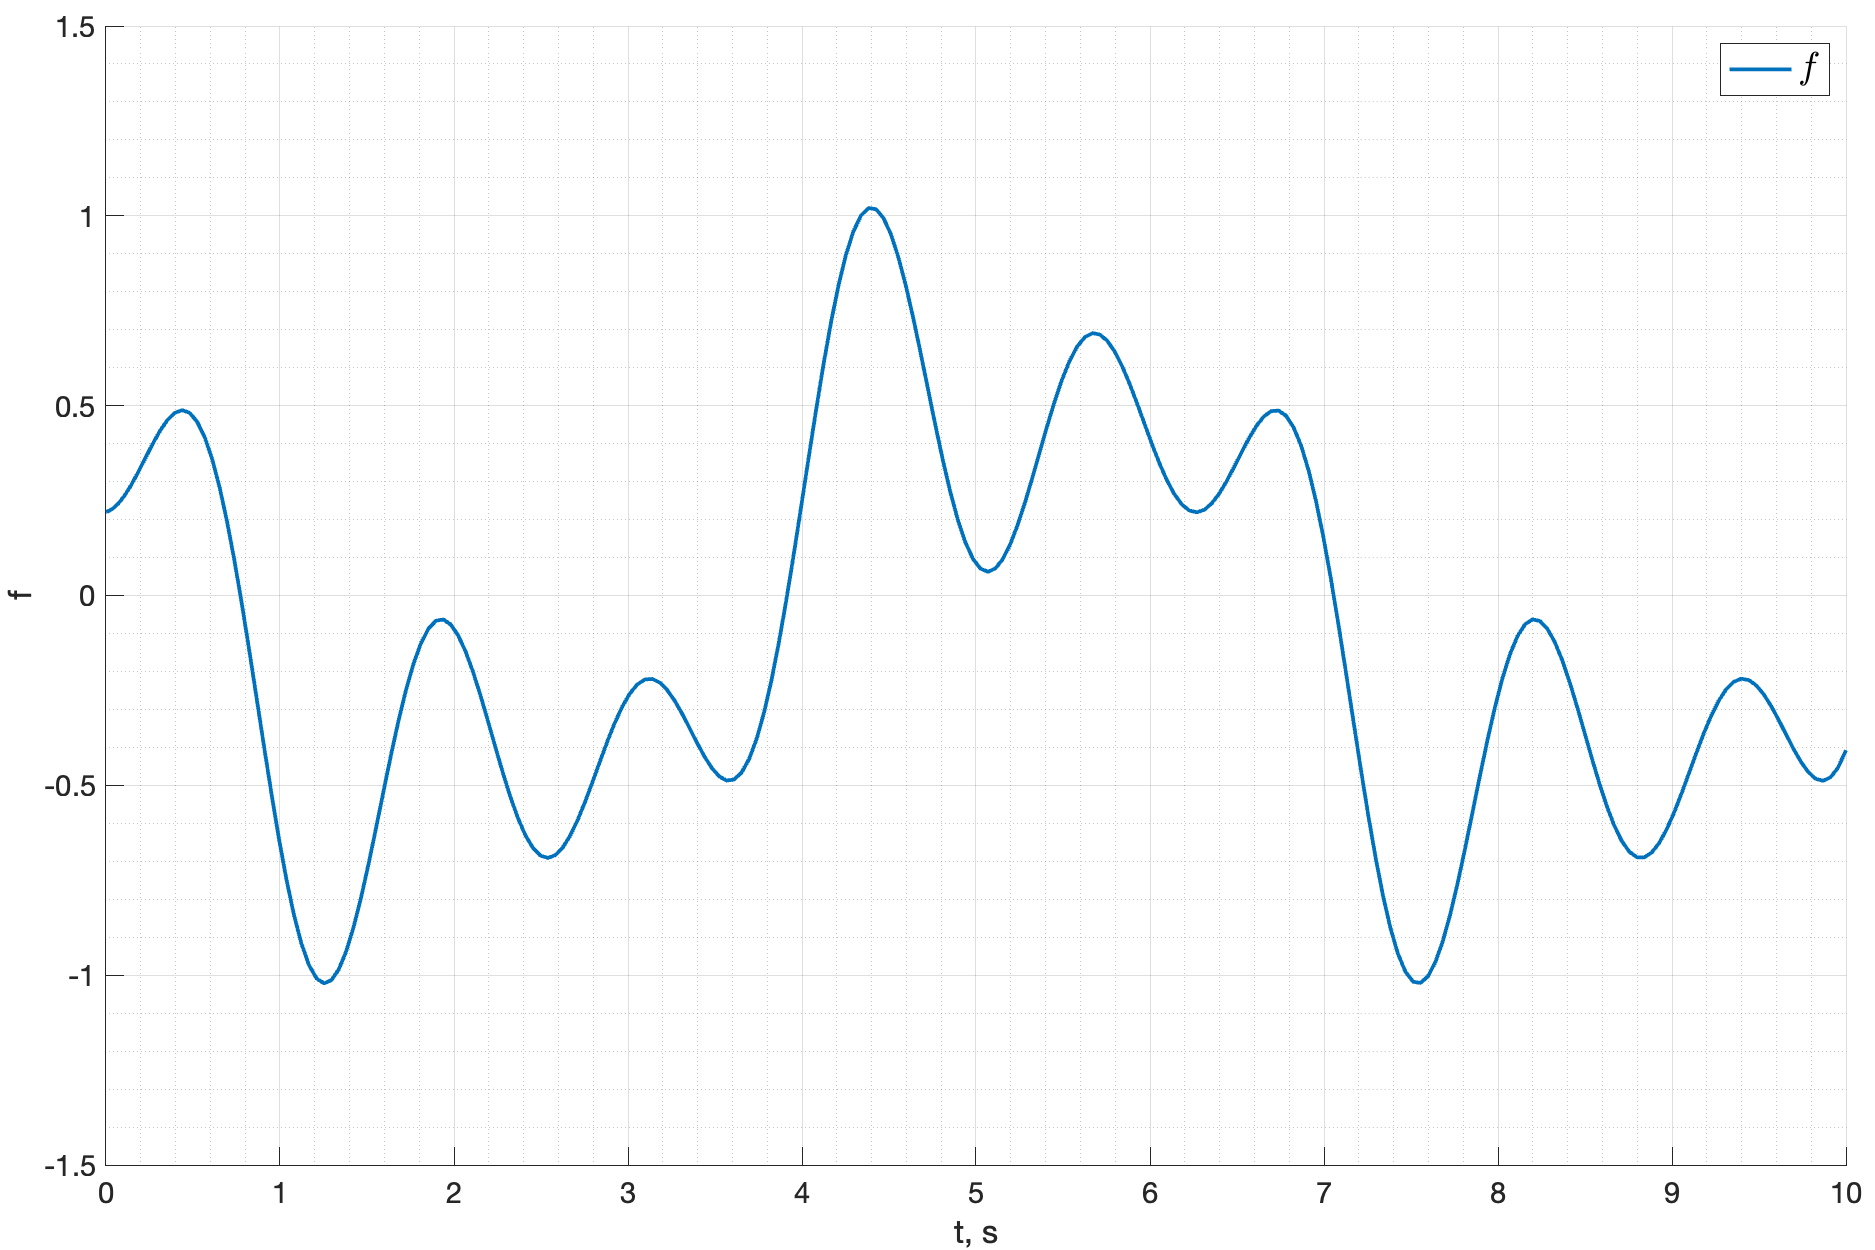
\includegraphics[width=\textwidth]{media/plots/compensation/force.png}
    \caption{График сгенерированного сигнала $f(t)$}
    \label{fig:signal_generation}
\end{figure}

\subsection{Компенсирующий регулятор}
Рассмотрим регулятор, способный компенсировать влияние внешнего возмущения $f(t)$ на систему. Пусть регулятор имеет вид:
\begin{equation}
    u(t) = Kx + K_f w_f 
\end{equation}
где $K$ -- feedback компонента, $K_f$ -- feedforward компонента. 

Для синтеза feedback компонентны будем использовать уже рассмотренный ранее метод LQR.
Для заданной степени устойчивости $\alpha = 2$ получает матрицу регулятора $K$:
\begin{eqnarray}
    K = \begin{bmatrix}
        8804.48  & 6658.07  & -23113.34  & -5271.36 \\ 
    \end{bmatrix}
\end{eqnarray}
С собственными числами замкнутой системы:
\begin{equation}
    \sigma(A + BK) = \begin{bmatrix}
        -3.63 + 6.93j \\ 
        -3.63 - 6.93j \\ 
        -4.38 \\ 
        -2.44 \\ 
    \end{bmatrix}
\end{equation}

Для синтеза feedforward компоненты $K_f$ рассмотрим систему:
\begin{equation}
    \begin{cases}
        P\Gamma_f - AP = BY + DY_f \\ 
        C_z P = 0 \\ 
        K_f = Y - K P \\ 
    \end{cases}
\end{equation}
где $C_z$ -- матрица виртуального выхода системы, обеспечивающий заданное условие 
сходимости угла отклонения маятника к нулю
\begin{equation}
    \lim_{t\to\infty} ||\theta|| = 0
\end{equation}
Условием существования такого регулятора является принадлежность собственных чисел 
внешнего возмущения правой комплексной полуплоскости и принадлежность корней 
системы, замкнутой регулятором, левой комплексной полуплоскости. Оба эти условия выполняются. 
Решим систему с помощью пакета \texttt{cvx} в MATLAB, в результате получаем:
\begin{equation}
    K_f = \begin{bmatrix}
190.03  & 2039.24  & 885.49  & 977.38  & -626.11  & 468.55  & -568.20  & 108.56  & 92.98  & -310.25 \\
    \end{bmatrix}
\end{equation}

\subsection{Моделирование}
Проведем моделирование линейной системы с полученным регулятором при наличии внешнего возмущения $f(t)$. 
Результат моделирования представлен на рисунке \ref{fig:compensation_lin}.
\begin{figure}[ht!]
    \centering
    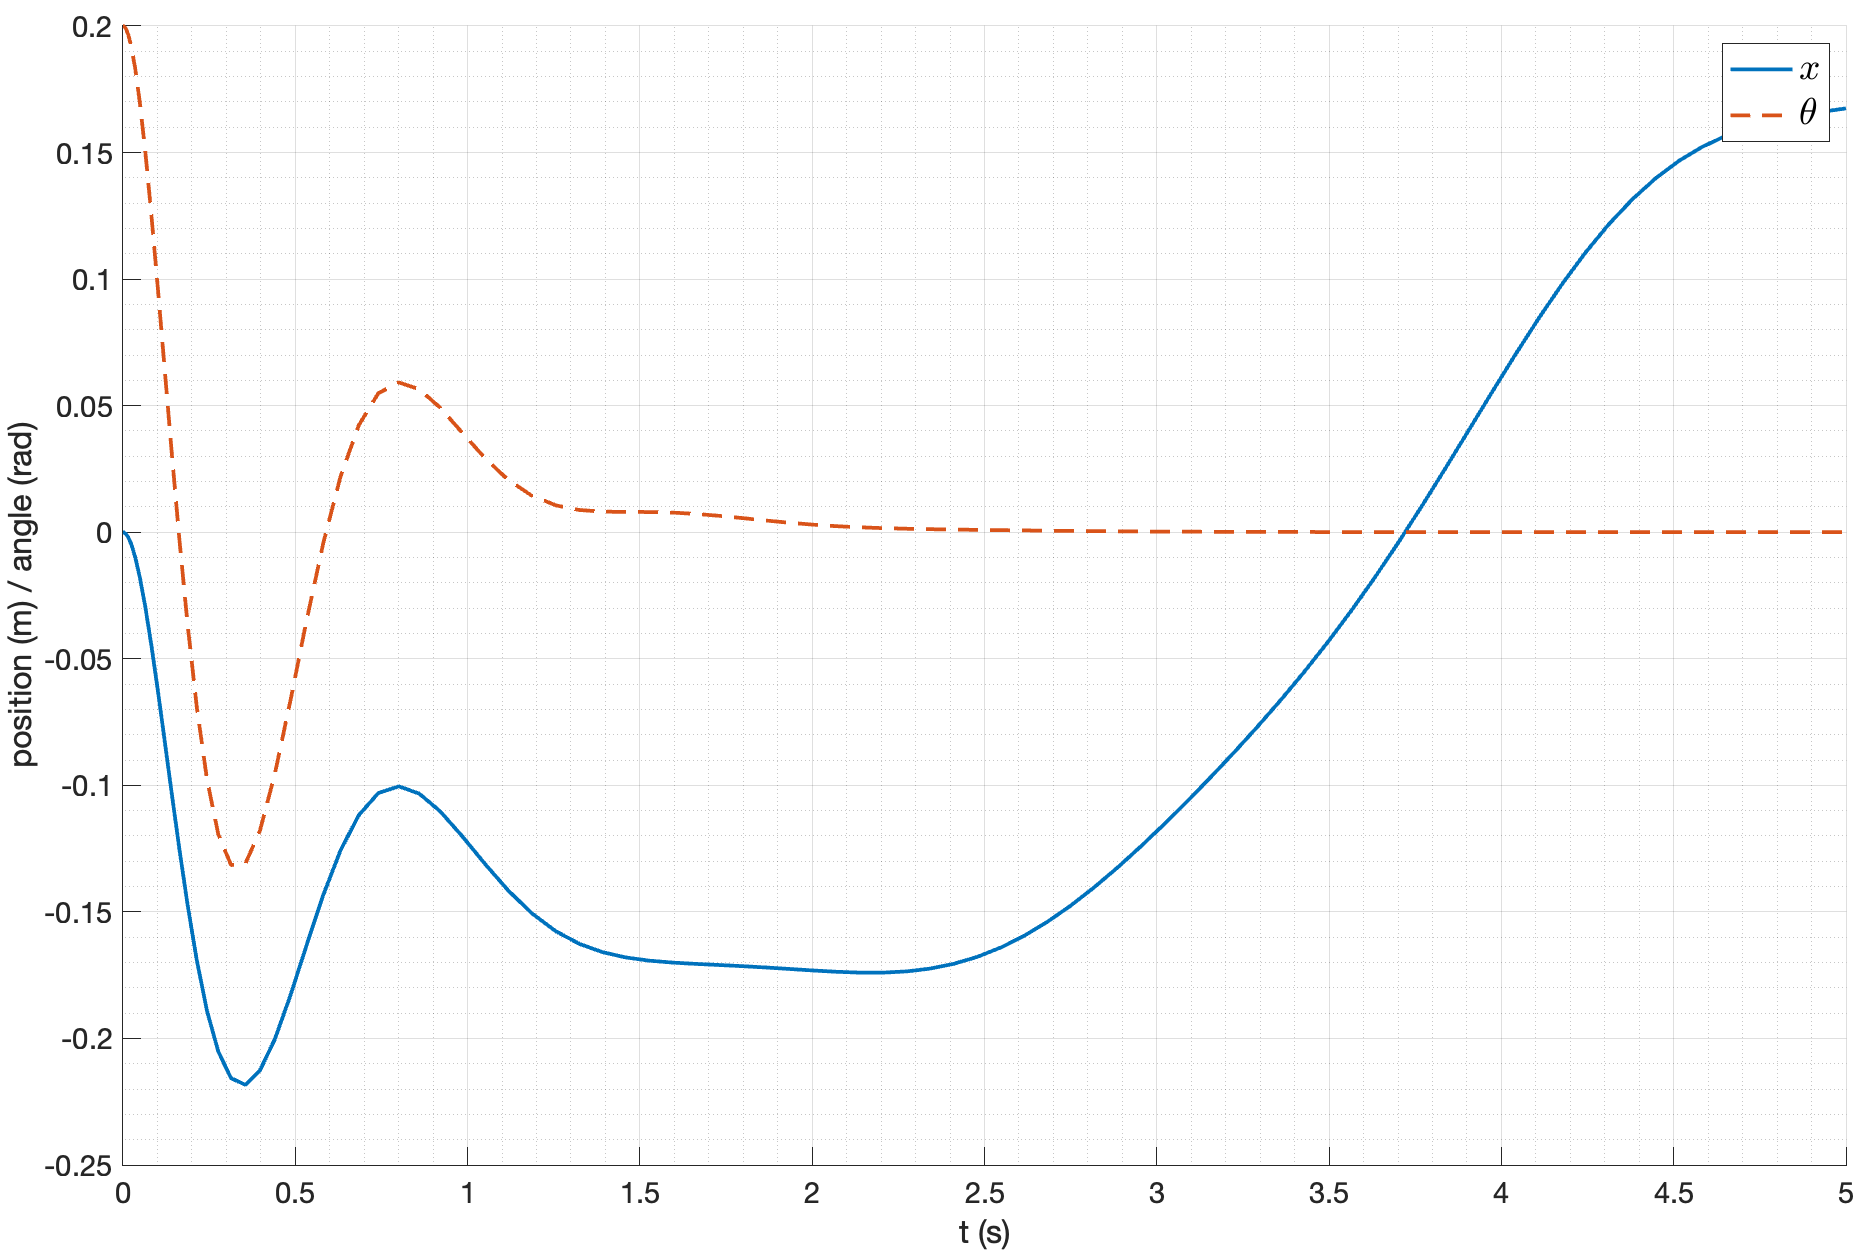
\includegraphics[width=\textwidth]{media/plots/compensation/linear_out_1.png}
    \caption{График выхода линейной системы с компенсирующим регулятором}
    \label{fig:compensation_lin}
\end{figure}
Видно, что как и было необходимо, угловое отклонение маятника стремится к нулю, при этом 
положение тележки не сходится к нулю. 

График изменение вектора состояние линейной системы с компенсирующим регулятором представлен на рисунке \ref{fig:compensation_lin_state}.
\begin{figure}[ht!]
    \centering
    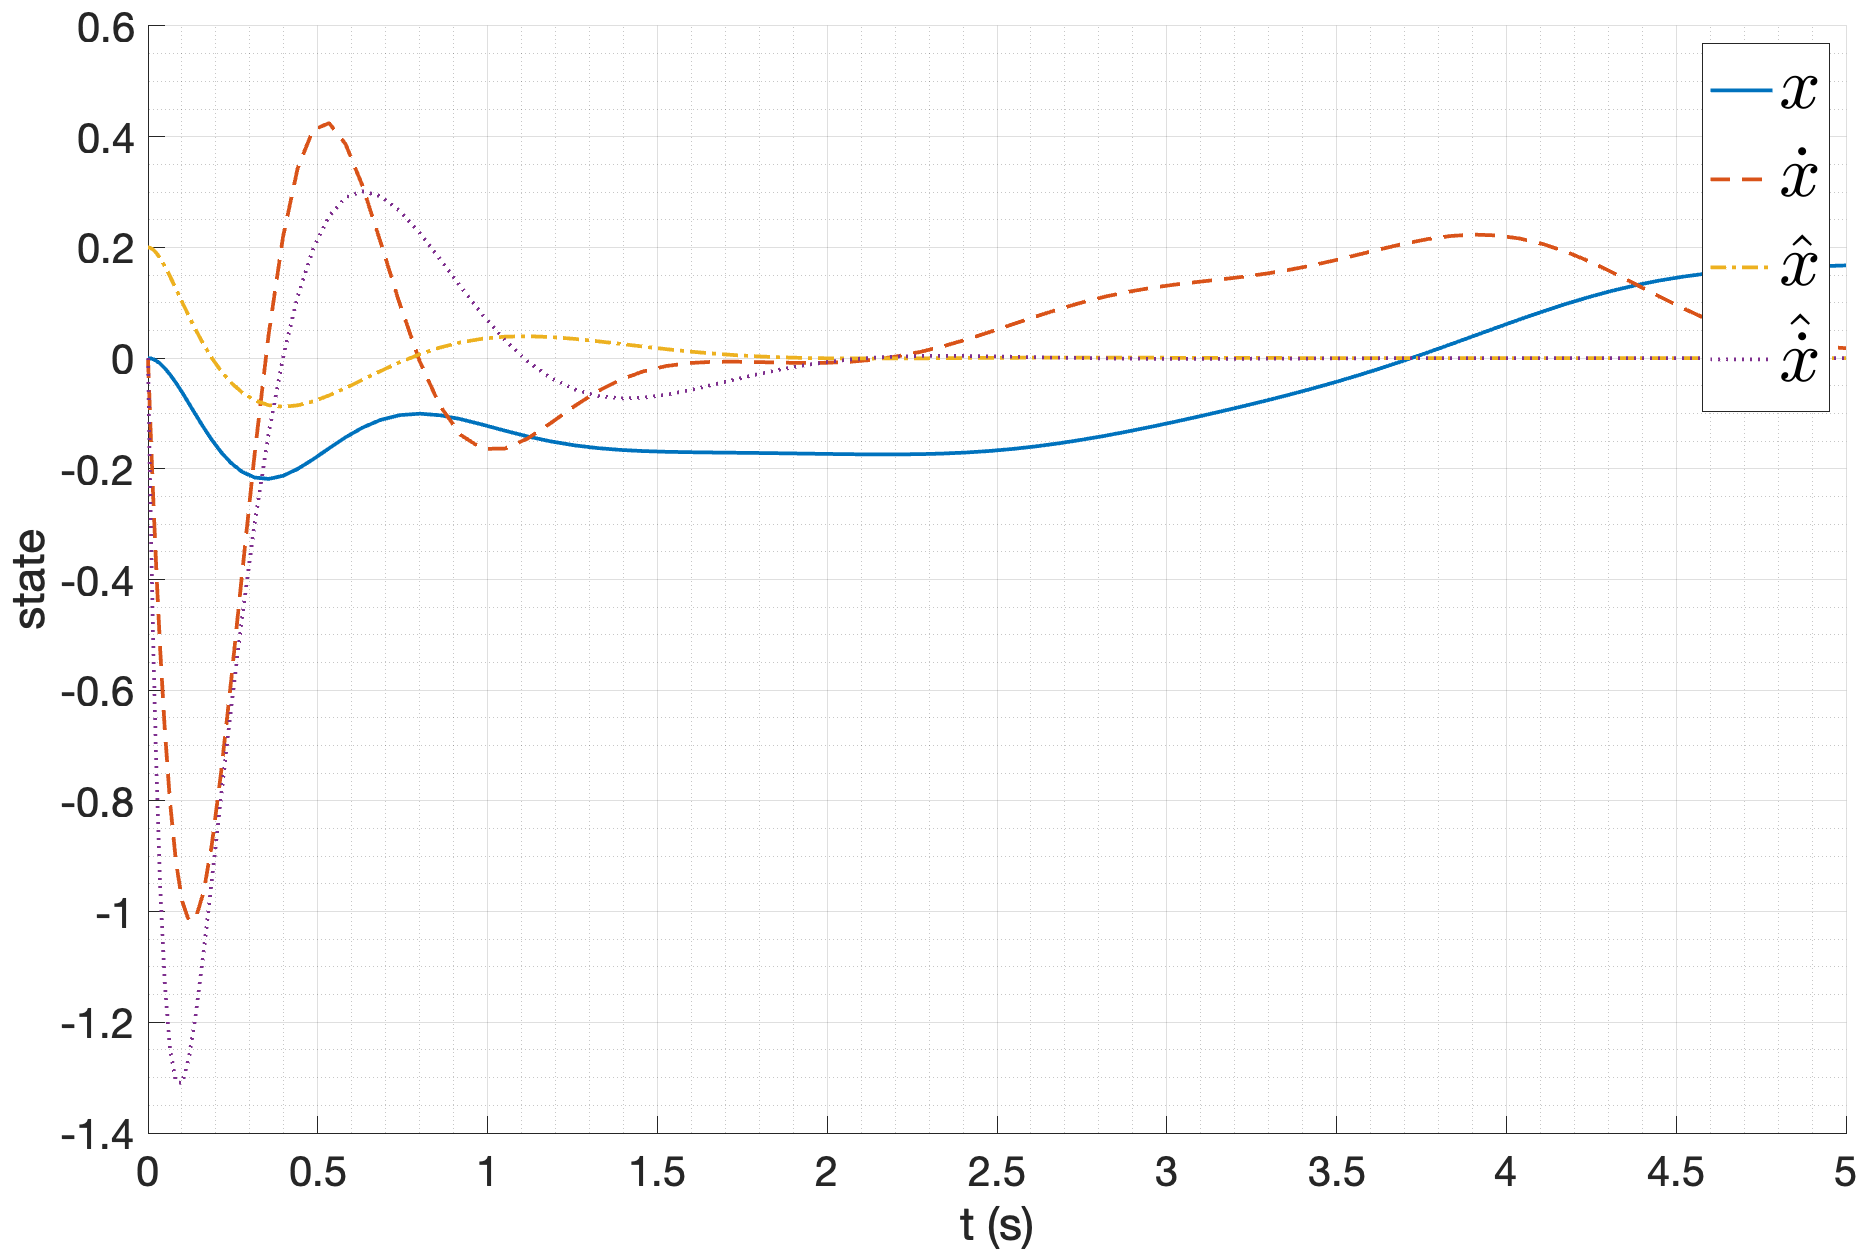
\includegraphics[width=0.8\textwidth]{media/plots/compensation/linear_state_1.png}
    \caption{График изменения вектора состояния линейной системы с компенсирующим регулятором}
    \label{fig:compensation_lin_state}
\end{figure}

Проведем моделирование нелинейной системы с полученным регулятором при наличии внешнего возмущения $f(t)$.
Результат моделирования представлен на рисунке \ref{fig:compensation_nlin}.
\begin{figure}[ht!]
    \centering
    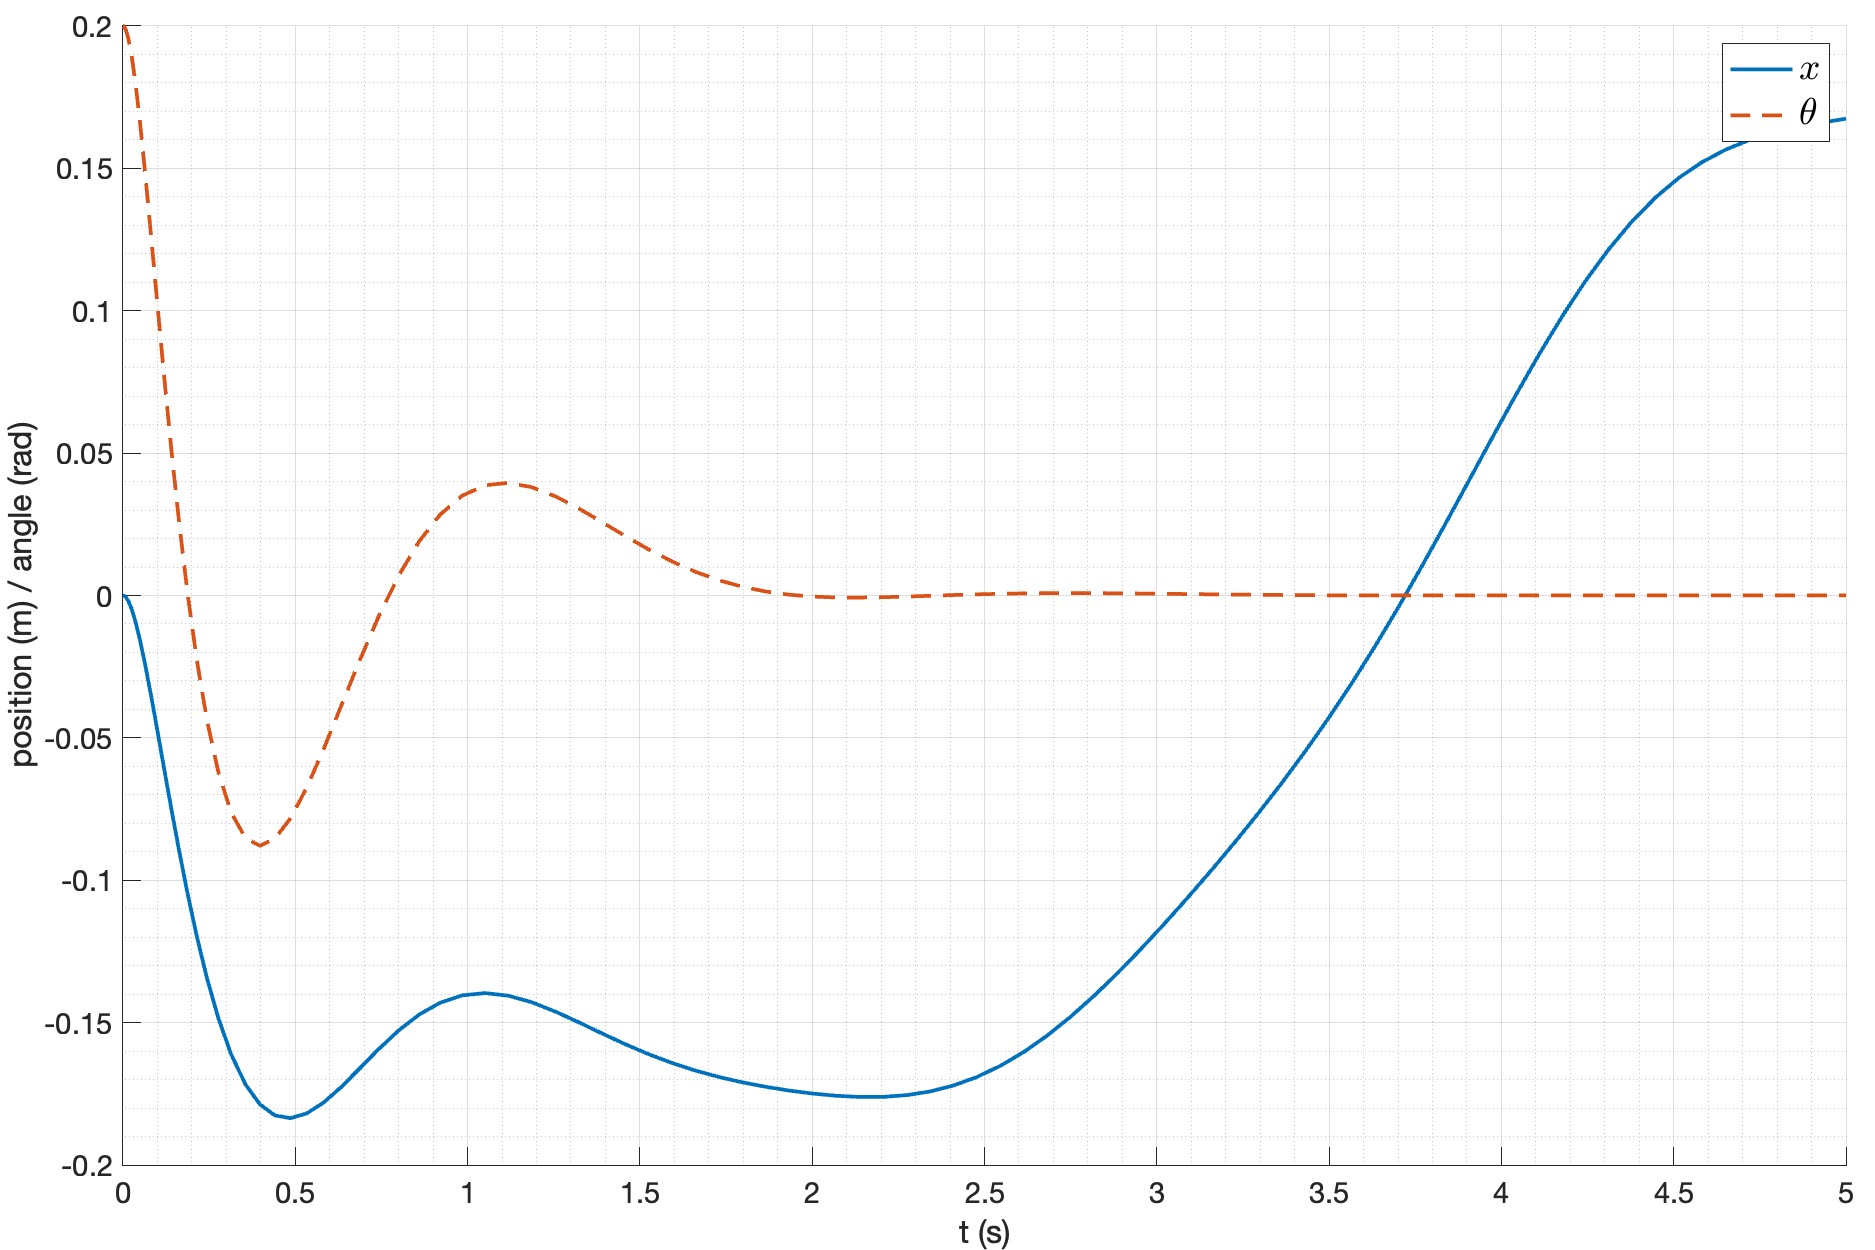
\includegraphics[width=0.8\textwidth]{media/plots/compensation/out_1.png}
    \caption{График выхода нелинейной системы с компенсирующим регулятором}
    \label{fig:compensation_nlin}
\end{figure}
Как и в случае линейной системы, угловое отклонение маятника стремится к нулю, при этом 
положение тележки не сходится к нулю. 
График изменение вектора состояние нелинейной системы с компенсирующим регулятором представлен на рисунке \ref{fig:compensation_nlin_state}.
\begin{figure}[ht!]
    \centering
    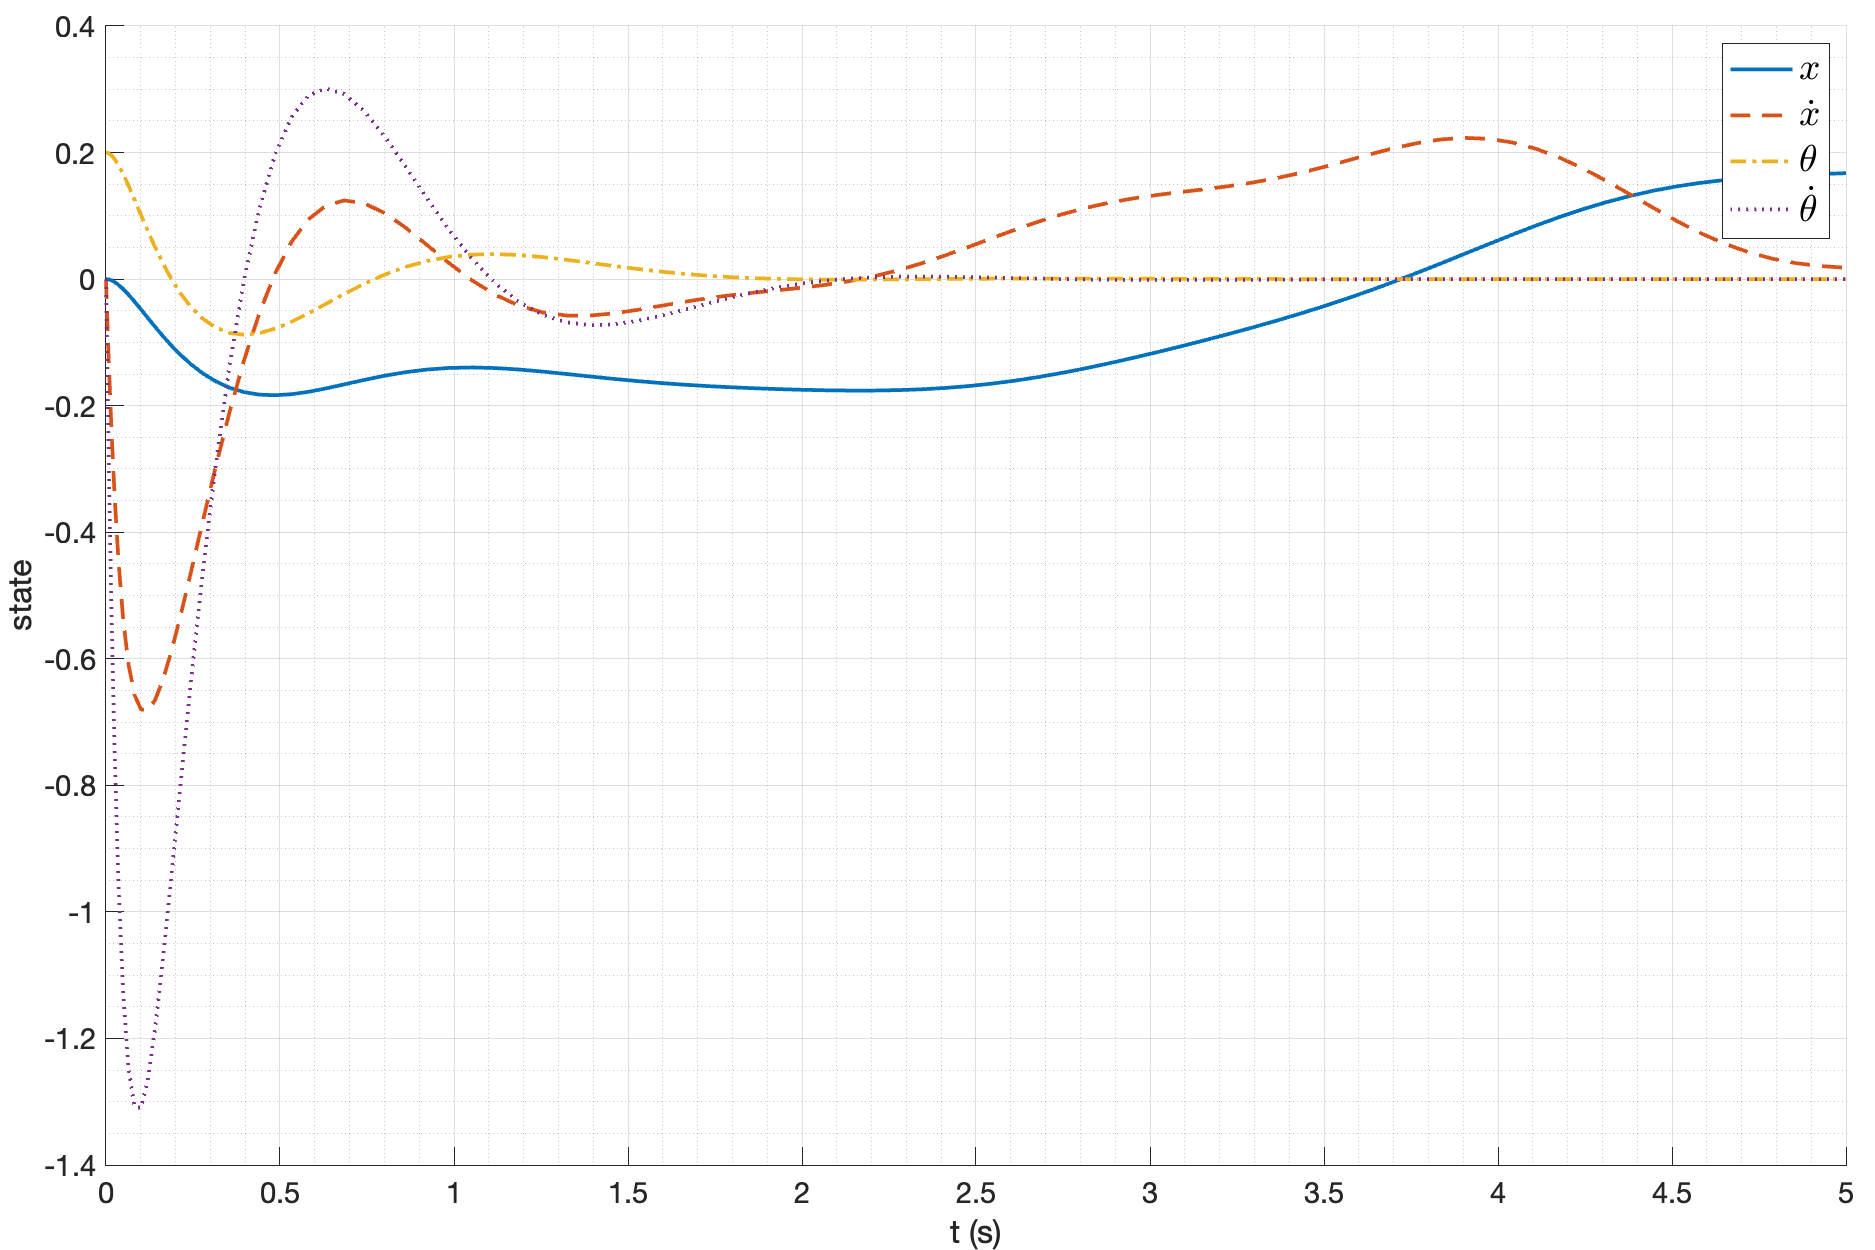
\includegraphics[width=0.8\textwidth]{media/plots/compensation/state_1.png}
    \caption{График изменения вектора состояния нелинейной системы с компенсирующим регулятором}
    \label{fig:compensation_nlin_state}
\end{figure}
График управляющего воздействия нелинейной системы с компенсирующим регулятором представлен на рисунке \ref{fig:compensation_nlin_control}.
\begin{figure}[ht!]
    \centering
    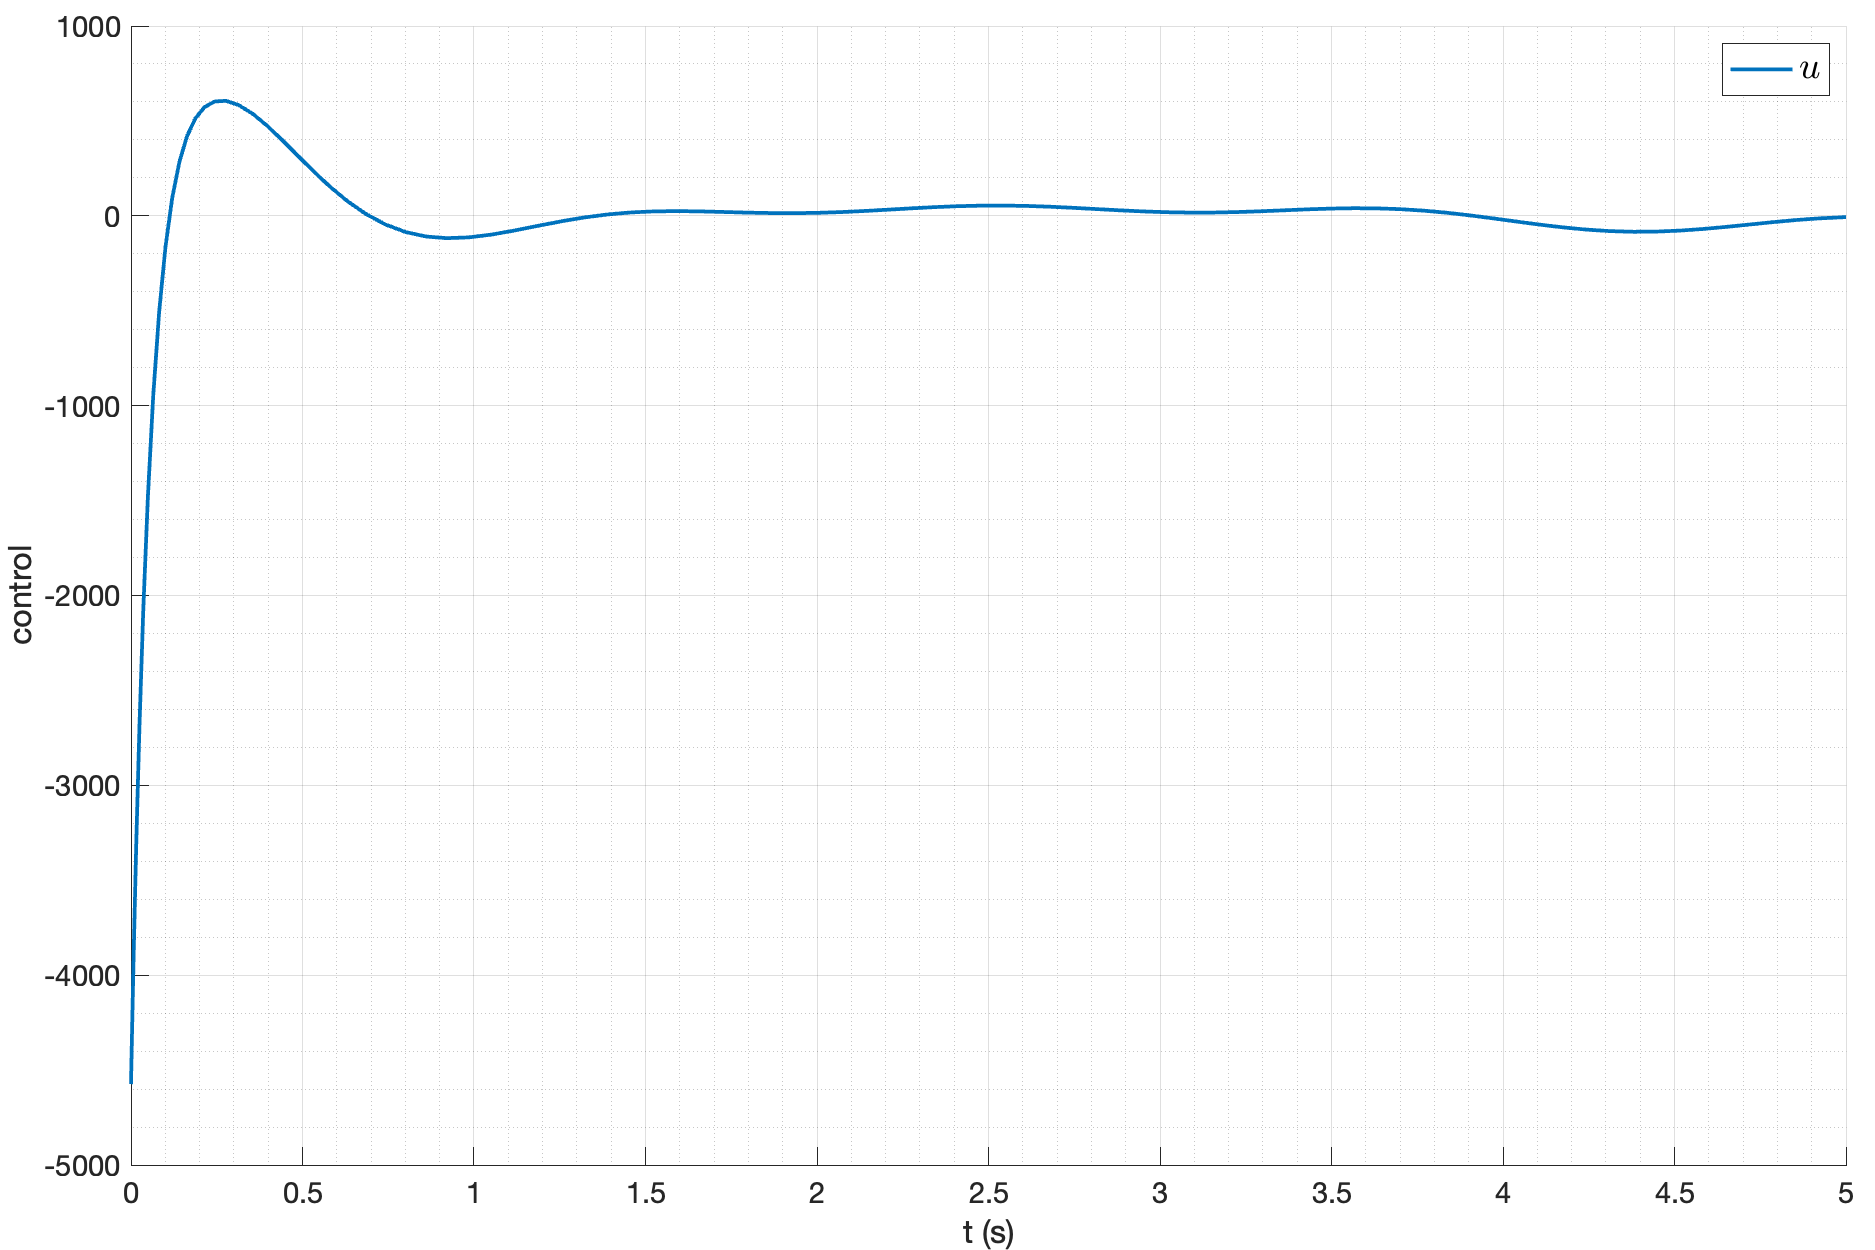
\includegraphics[width=0.8\textwidth]{media/plots/compensation/u_1.png}
    \caption{График управляющего воздействия нелинейной системы с компенсирующим регулятором}
    \label{fig:compensation_nlin_control}
\end{figure}
\FloatBarrier
Таким образом, полученный регулятор успешно справляется с компенсацией внешнего возмущения $f(t)$,
условие сходимости угла отклонения маятника к нулю выполняется, при этом положение тележки не стремится к нулю.
Полученный регулятор работает корректно как в линейной, так и в нелинейной системе. 

\subsection{Слежение за внешним возмущением}
Возьмем тот же сигнал $g(t) = f(t)$, что и в предыдущем пункте, и рассмотрим систему слежения за этим сигналом:  
\begin{equation}
    \lim_{t\to\infty} ||\theta(t) - g(t)|| = 0
\end{equation}
регулятор будет иметь вид:
\begin{equation}
    u(t) = Kx + K_g w_f
\end{equation}
В качестве feedback компоненты $K$ будем использовать уже рассмотренный ранее регулятор LQR: 
\begin{eqnarray}
    K = \begin{bmatrix}
        8804.48  & 6658.07  & -23113.34  & -5271.36 \\ 
    \end{bmatrix}
\end{eqnarray}
Для синтеза feedforward компоненты $K_g$ рассмотрим систему:
\begin{equation}
    \begin{cases}
        P\Gamma_f - AP = BY \\
        C_z P - Y_g = 0 \\
        K_g = Y - K P \\
    \end{cases}
\end{equation}
Решив систему с помощью пакета \texttt{cvx} в MATLAB, получаем:
\begin{equation}
    K_g = \begin{bmatrix}
        -10582  & -54283  & -27722  & -11896  & 1774  & -16672  & 2018  & -12144  & 6860  & 1718 \\ 
    \end{bmatrix}
\end{equation}
\subsection{Моделирование}
Проведем моделирование линейной системы с полученным регулятором для слежения за задающим сигналом $g(t)$.
Результат моделирования представлен на рисунке \ref{fig:tracking_lin}.
\begin{figure}[ht!]
    \centering
    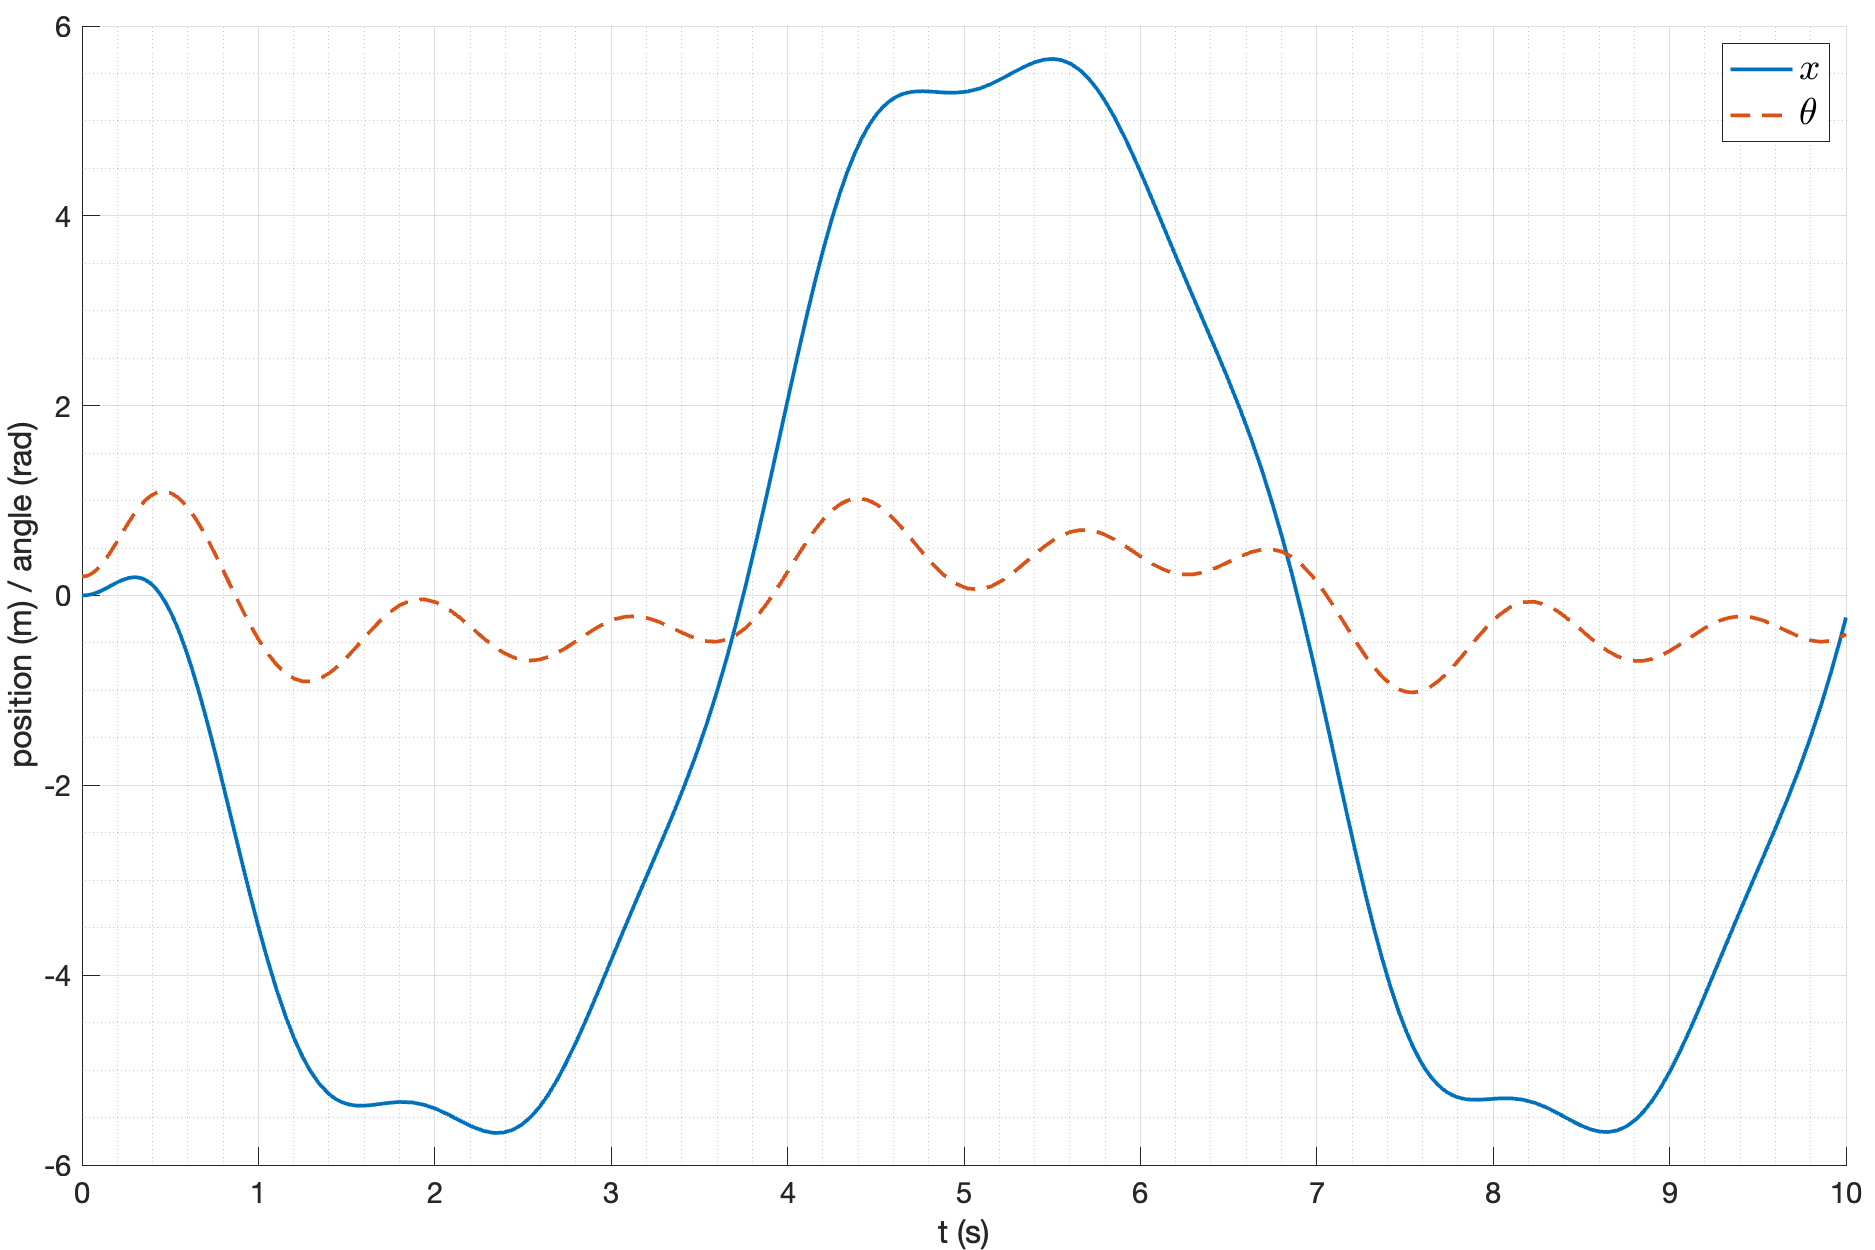
\includegraphics[width=0.8\textwidth]{media/plots/follow/linear_out_1.png}
    \caption{График выхода линейной системы с регулятором слежения}
    \label{fig:tracking_lin}
\end{figure}
Построим график угла отклонения маятника и задающего сигнала $g(t)$ на одном графике для наглядности.
Результат представлен на рисунке \ref{fig:tracking_lin_cmp}.
\begin{figure}[ht!]
    \centering
    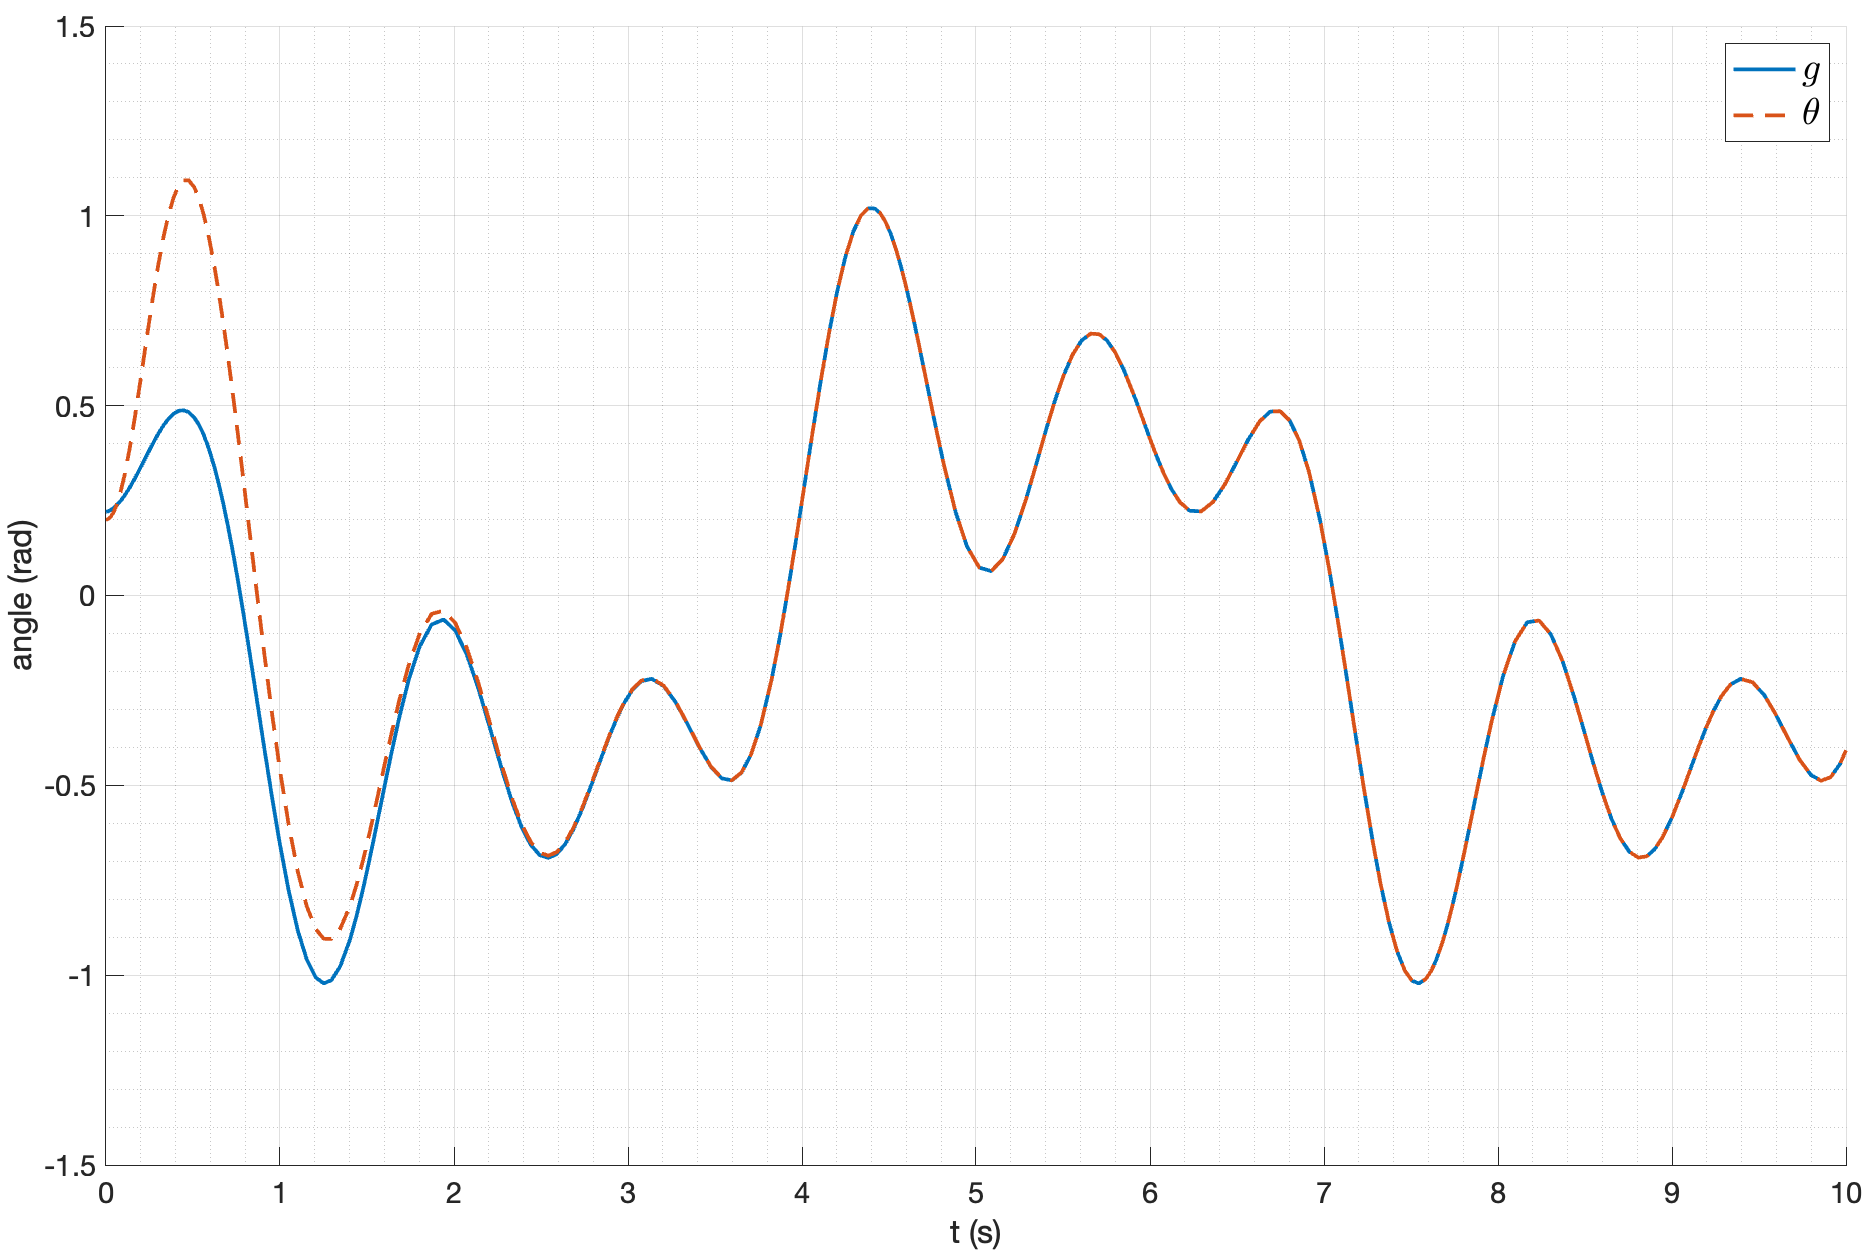
\includegraphics[width=0.8\textwidth]{media/plots/follow/linear_cmp1.png}
    \caption{График угла отклонения маятника и задающего сигнала $g(t)$}
    \label{fig:tracking_lin_cmp}
\end{figure}
Видно, что угол отклонения маятника стремится повторить задающий сигнал $g(t)$, убедиться 
с этом можно посмотрев на график ошибки слежения на рисунке \ref{fig:tracking_lin_err}. 
\begin{figure}[ht!]
    \centering
    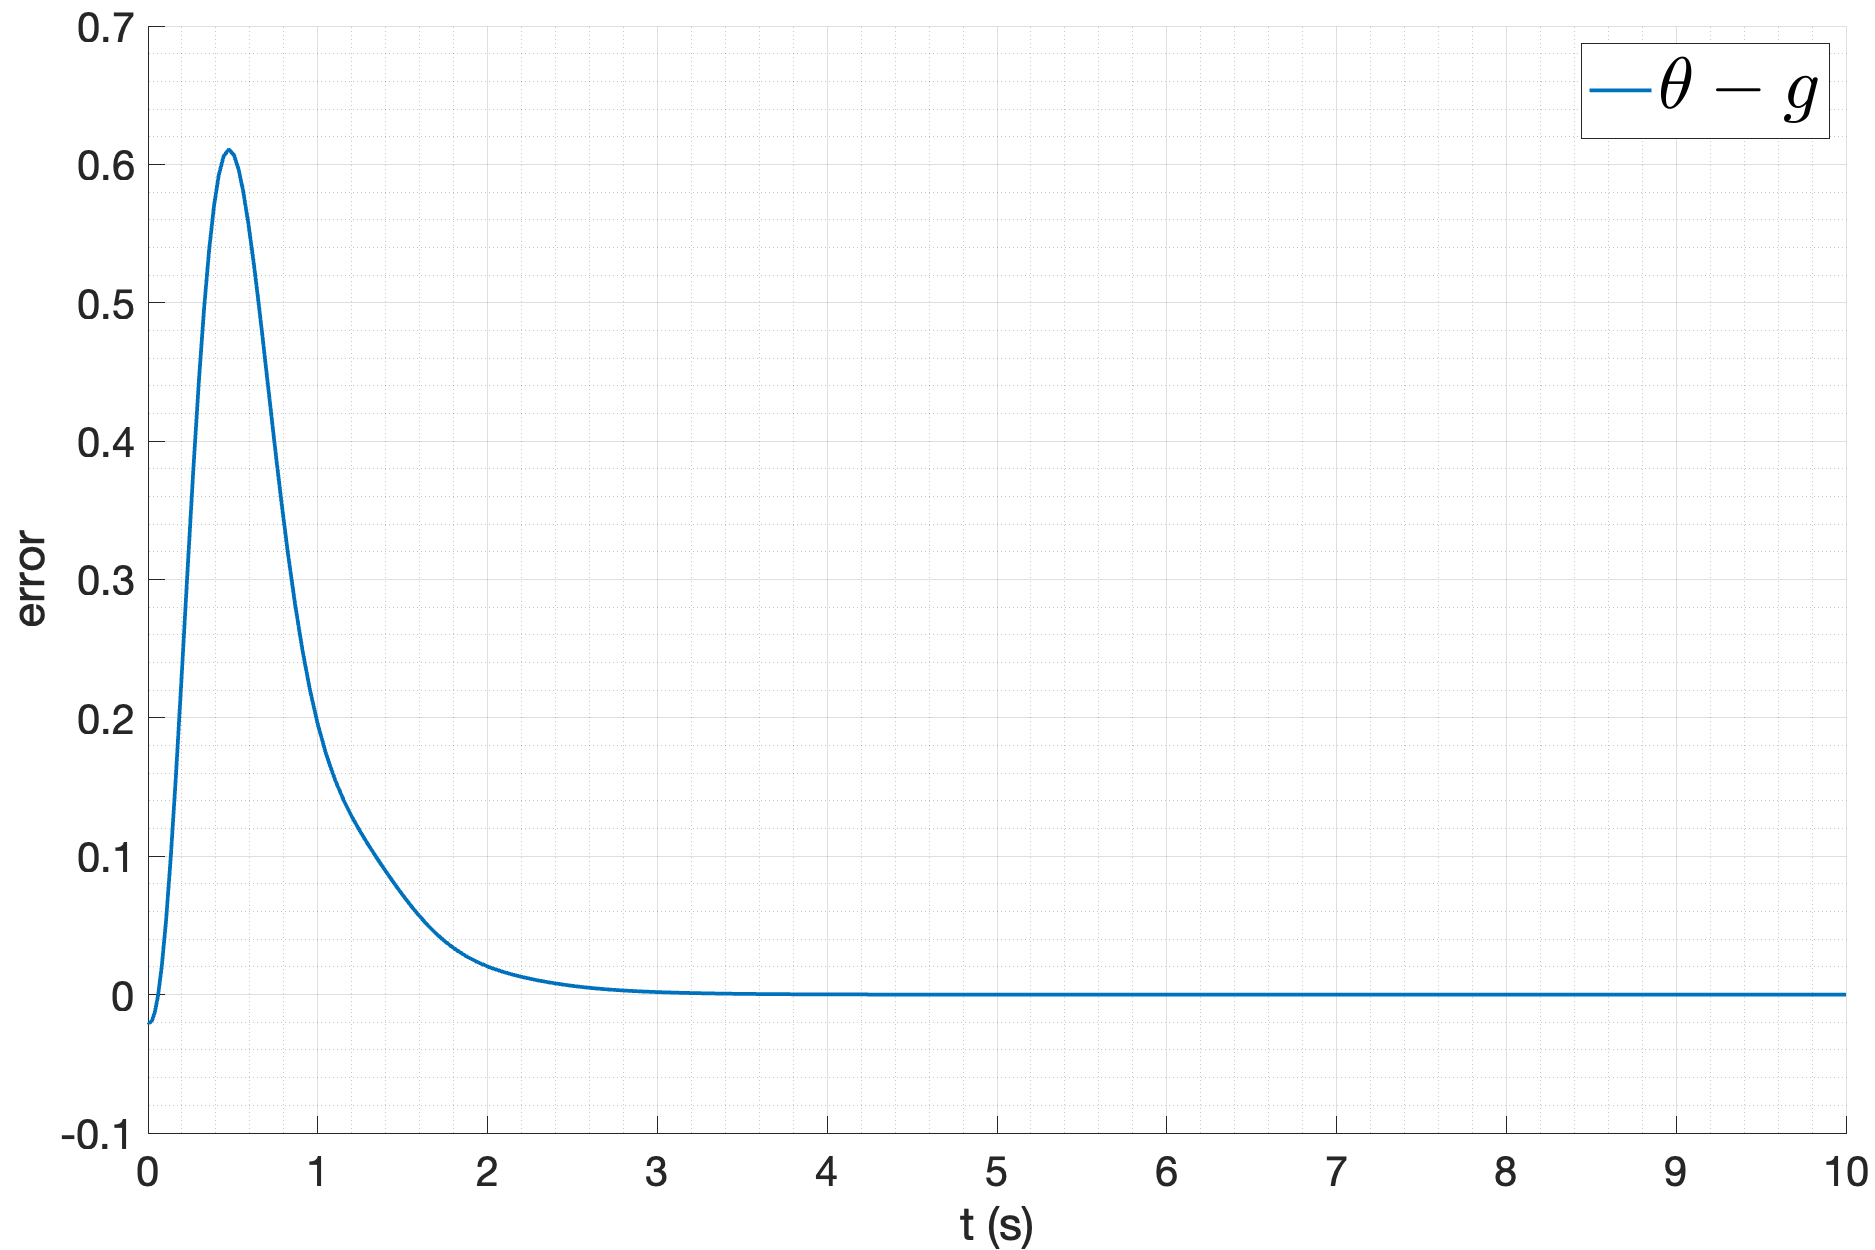
\includegraphics[width=0.8\textwidth]{media/plots/follow/linear_error_1.png}
    \caption{График ошибки слежения линейной системы}
    \label{fig:tracking_lin_err}
\end{figure}
Ошибки сходится к нулю, что подтверждает корректность работы регулятора. 

\FloatBarrier
Проверим работоспособность регулятора в нелинейной системе. Результат моделирования представлен на рисунке \ref{fig:tracking_nlin}.
\begin{figure}[ht!]
    \centering
    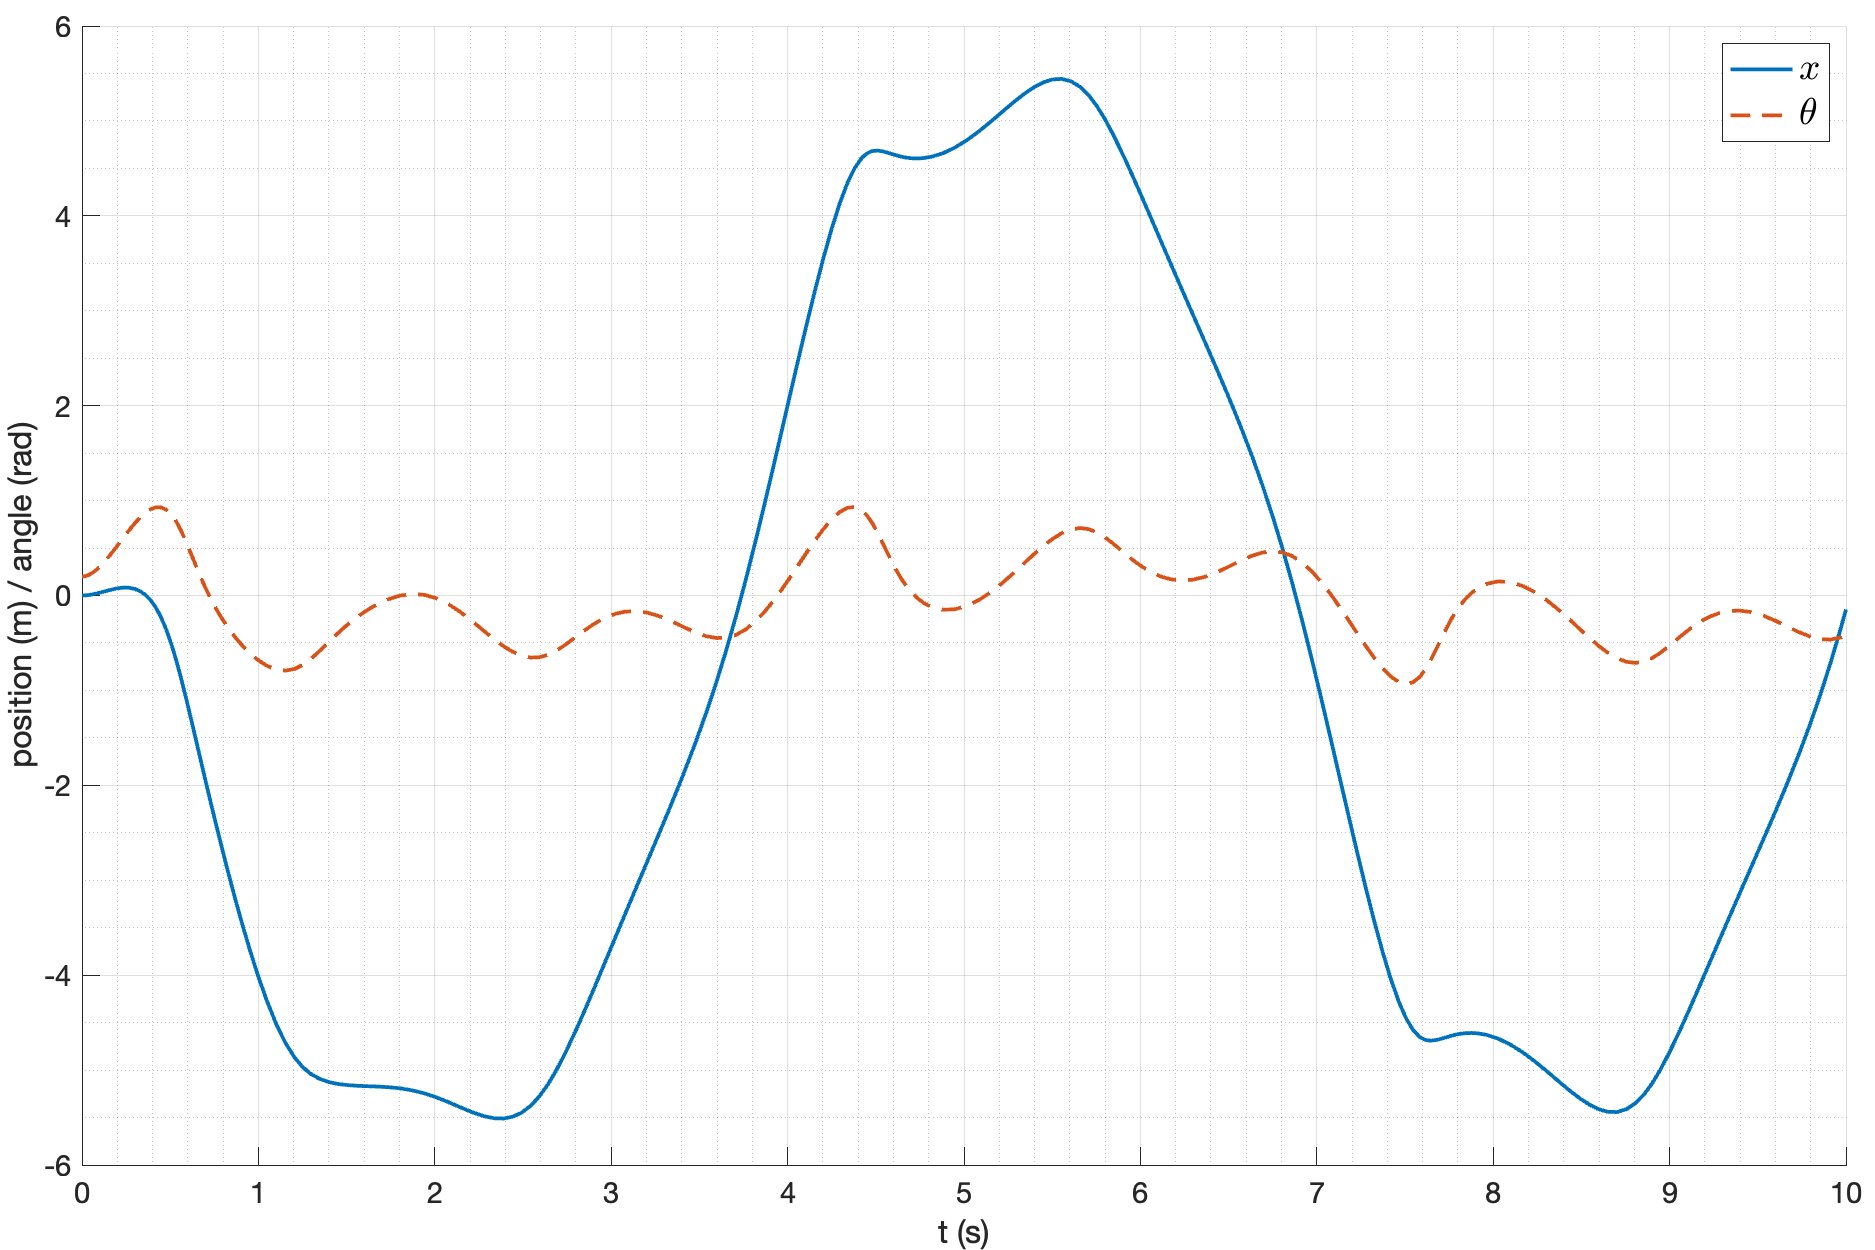
\includegraphics[width=0.8\textwidth]{media/plots/follow/out_1.png}
    \caption{График выхода нелинейной системы с регулятором слежения}
    \label{fig:tracking_nlin}
\end{figure}
Построим график угла отклонения маятника и задающего сигнала $g(t)$ на одном графике для наглядности и 
график ошибки слежения на рисунке \ref{fig:tracking_nlin_err}.
Результат представлен на рисунке \ref{fig:tracking_nlin_cmp}.
\begin{figure}[ht!]
    \centering
    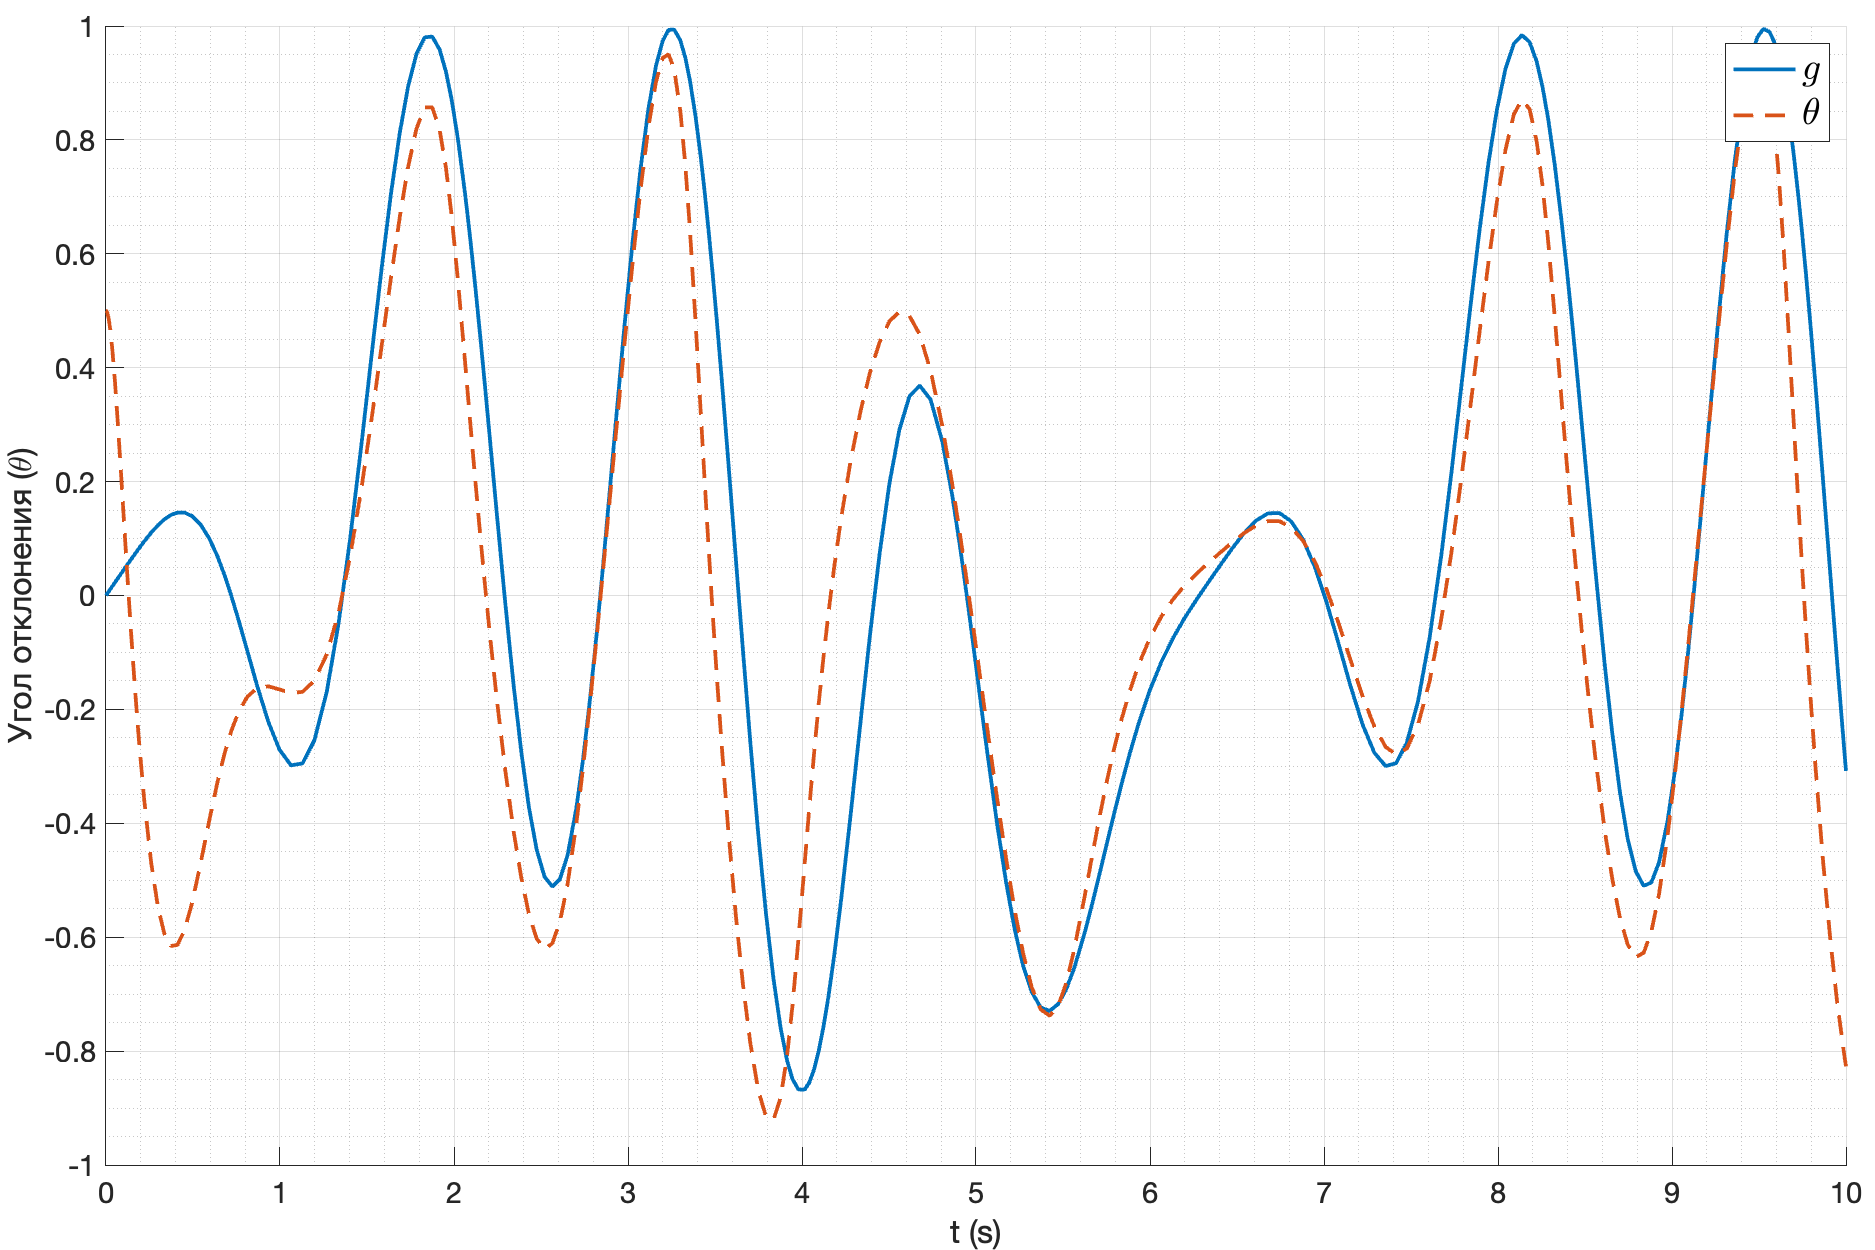
\includegraphics[width=0.8\textwidth]{media/plots/follow/cmp_1.png}
    \caption{График угла отклонения маятника и задающего сигнала $g(t)$}
    \label{fig:tracking_nlin_cmp}
\end{figure}
\begin{figure}[ht!]
    \centering
    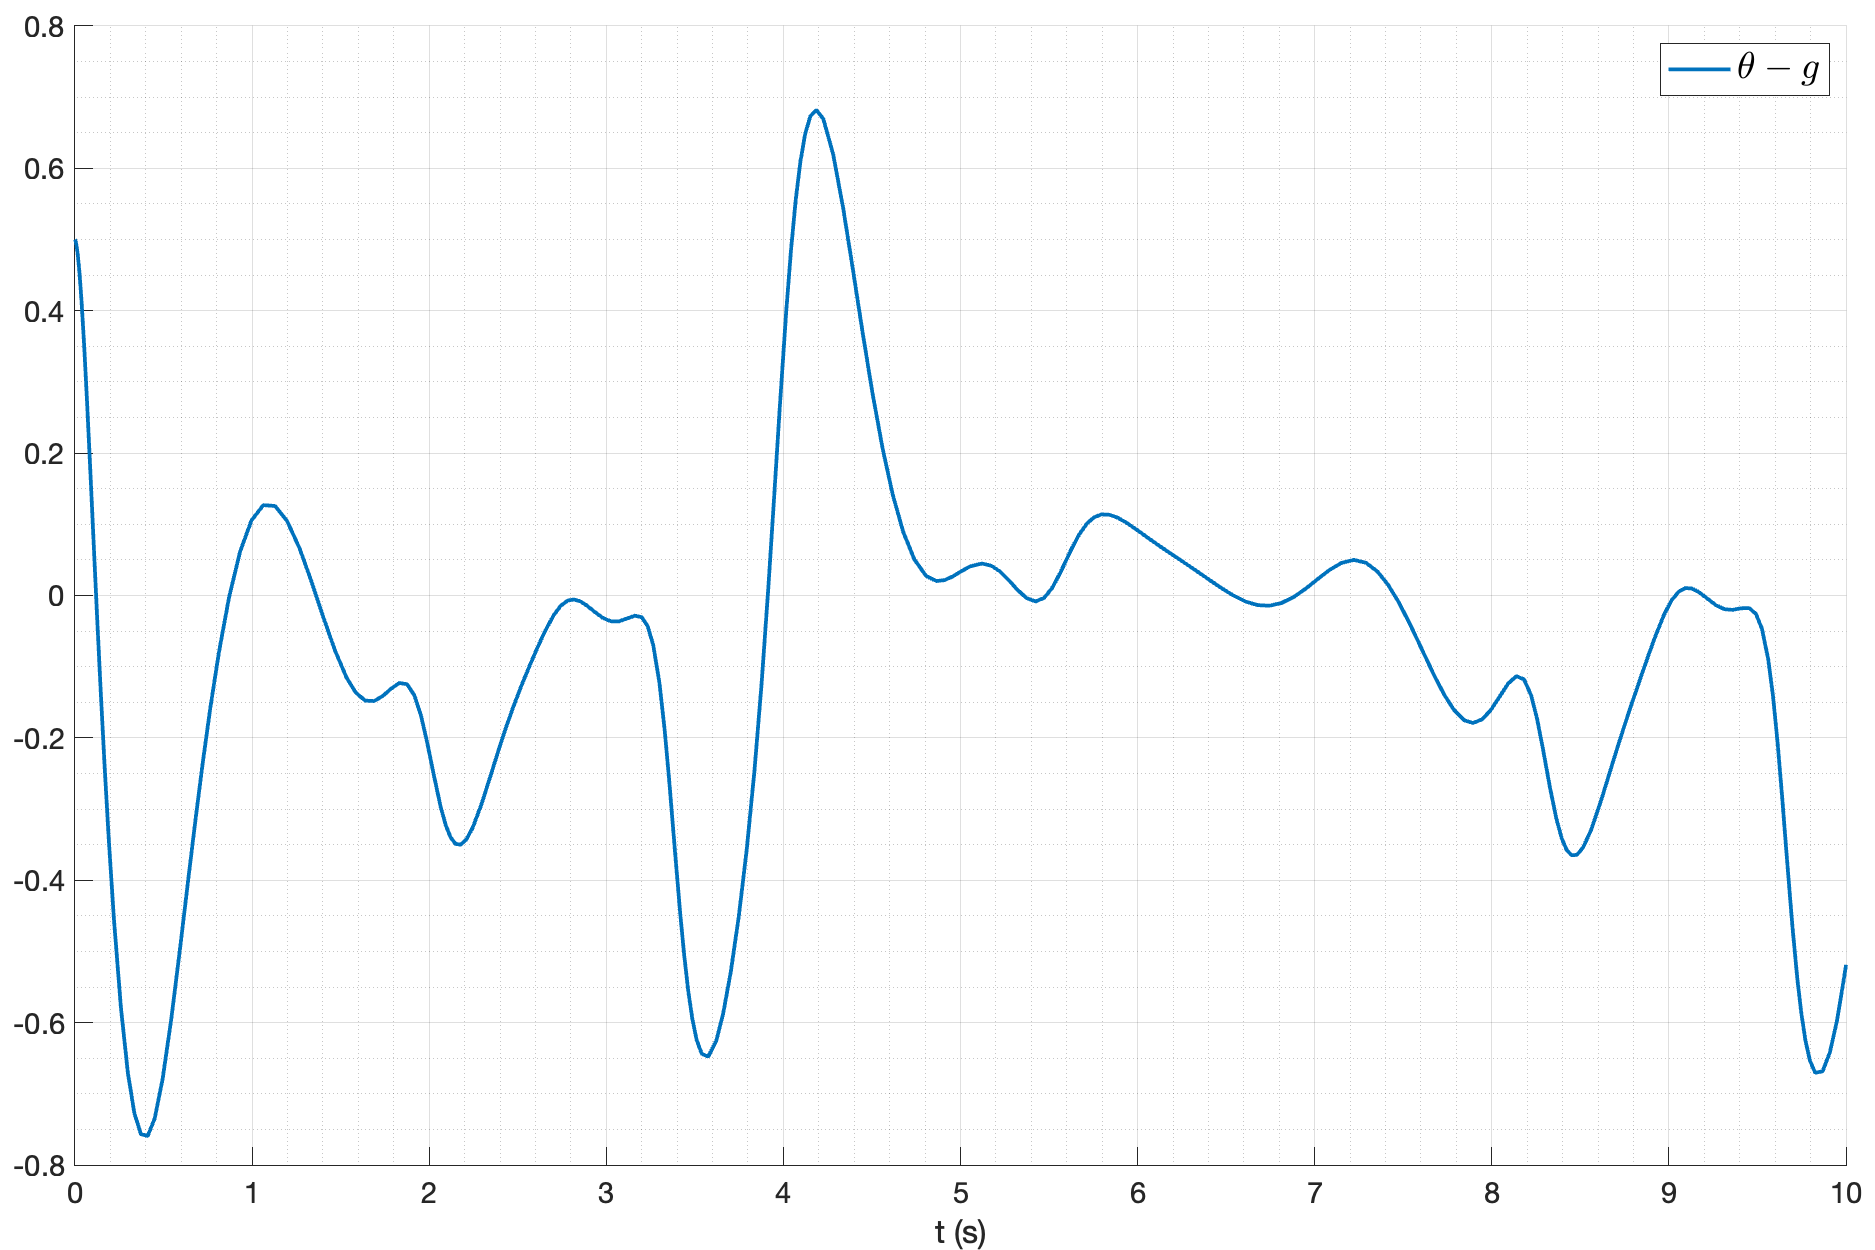
\includegraphics[width=0.8\textwidth]{media/plots/follow/error_1.png}
    \caption{График ошибки слежения нелинейной системы}
    \label{fig:tracking_nlin_err}
\end{figure}
Видно, что в случае нелинейной систему регулятор не справляется с задачей слежения за внешним возмущением $g(t)$, 
ошибка слежения не стремится к нулю. Это может быть связано с тем, что в нелинейной системе возникают дополнительные нелинейные эффекты, которые не учитываются в модели.

\subsection{Выводы}
В данной главе была рассмотрена задача компенсации внешнего возмущения и слежения за внешним возмущением. 
Полученные регулятора успешно справляются с задачей компенсации внешнего возмущения в линейной и нелинейной системах 
примерно одинаково, при этом условие сходимости угла отклонения маятника к нулю выполняется, что подтверждается результатами моделирования.
Однако, в случае слежения за внешним возмущением регулятор не справляется с задачей в нелинейной системе, что может быть связано с дополнительными нелинейными эффектами, которые не учитываются в модели, 
так как линейная модель дает корректные результаты только вблизи точки равновесия, а по графикам видно, что система отклоняется от точки равновесия довольно сильно. 